\documentclass[12pt]{report}
\usepackage[subpreambles=true]{standalone}
\usepackage[utf8]{inputenc}
\usepackage[english, polish]{babel}
\let\lll\undefined
\usepackage{import}

\usepackage[T1]{fontenc}
\usepackage[utf8]{inputenc}
\usepackage{graphicx}
\usepackage{amsmath,amssymb,amsfonts}
\usepackage{txfonts}
\usepackage{pdfpages}
\usepackage{afterpage}
\usepackage{lipsum}
\pagestyle{headings}
\usepackage{mathptmx}
\usepackage[font=small,labelfont={bf,it},textfont={it},justification=centering,skip=2pt]{caption}
\usepackage[backend=biber,sorting=none,style=numeric,giveninits=true,doi=false,url=false]{biblatex}
\usepackage[autostyle]{csquotes}
\usepackage{nameref}
\usepackage[parfill]{parskip}
\usepackage{url}
\usepackage{subcaption}

\addbibresource{bibliography.bib}
\addbibresource{website_bibliography.bib}

\newcommand\blankpage{%
    \null
    \thispagestyle{empty}%
    \addtocounter{page}{-1}%
    \newpage}
\newcommand*{\captionsource}[2]{%
  \caption[{#1}]{%
    #1%
    \\\textbf{Source:} #2
  }%
}


\DeclareMathOperator*{\argmax}{arg\,max}
\DeclareMathOperator*{\argmin}{arg\,min}
\DeclareMathAlphabet{\pazocal}{OMS}{zplm}{m}{n}
\DeclareQuoteStyle{polish}%
  {\textquoteleft}
  {\textquoteright}
  [0.05em]
  {\textquotedblleft}
  {\textquotedblright}

\setlength{\textwidth}{14cm}
\setlength{\textheight}{20cm}
\setlength{\parskip}{1em}
\renewcommand{\baselinestretch}{1.5}
\graphicspath{ {./images/} }


\title{Semantic image segmentation with use of conditional random fields}
\author{Aneta Andrzejewska}
\date{March 2019}

\begin{document}

\thispagestyle{empty}%
\addtocounter{page}{-1}%
\begin{titlepage}
\afterpage{\blankpage}
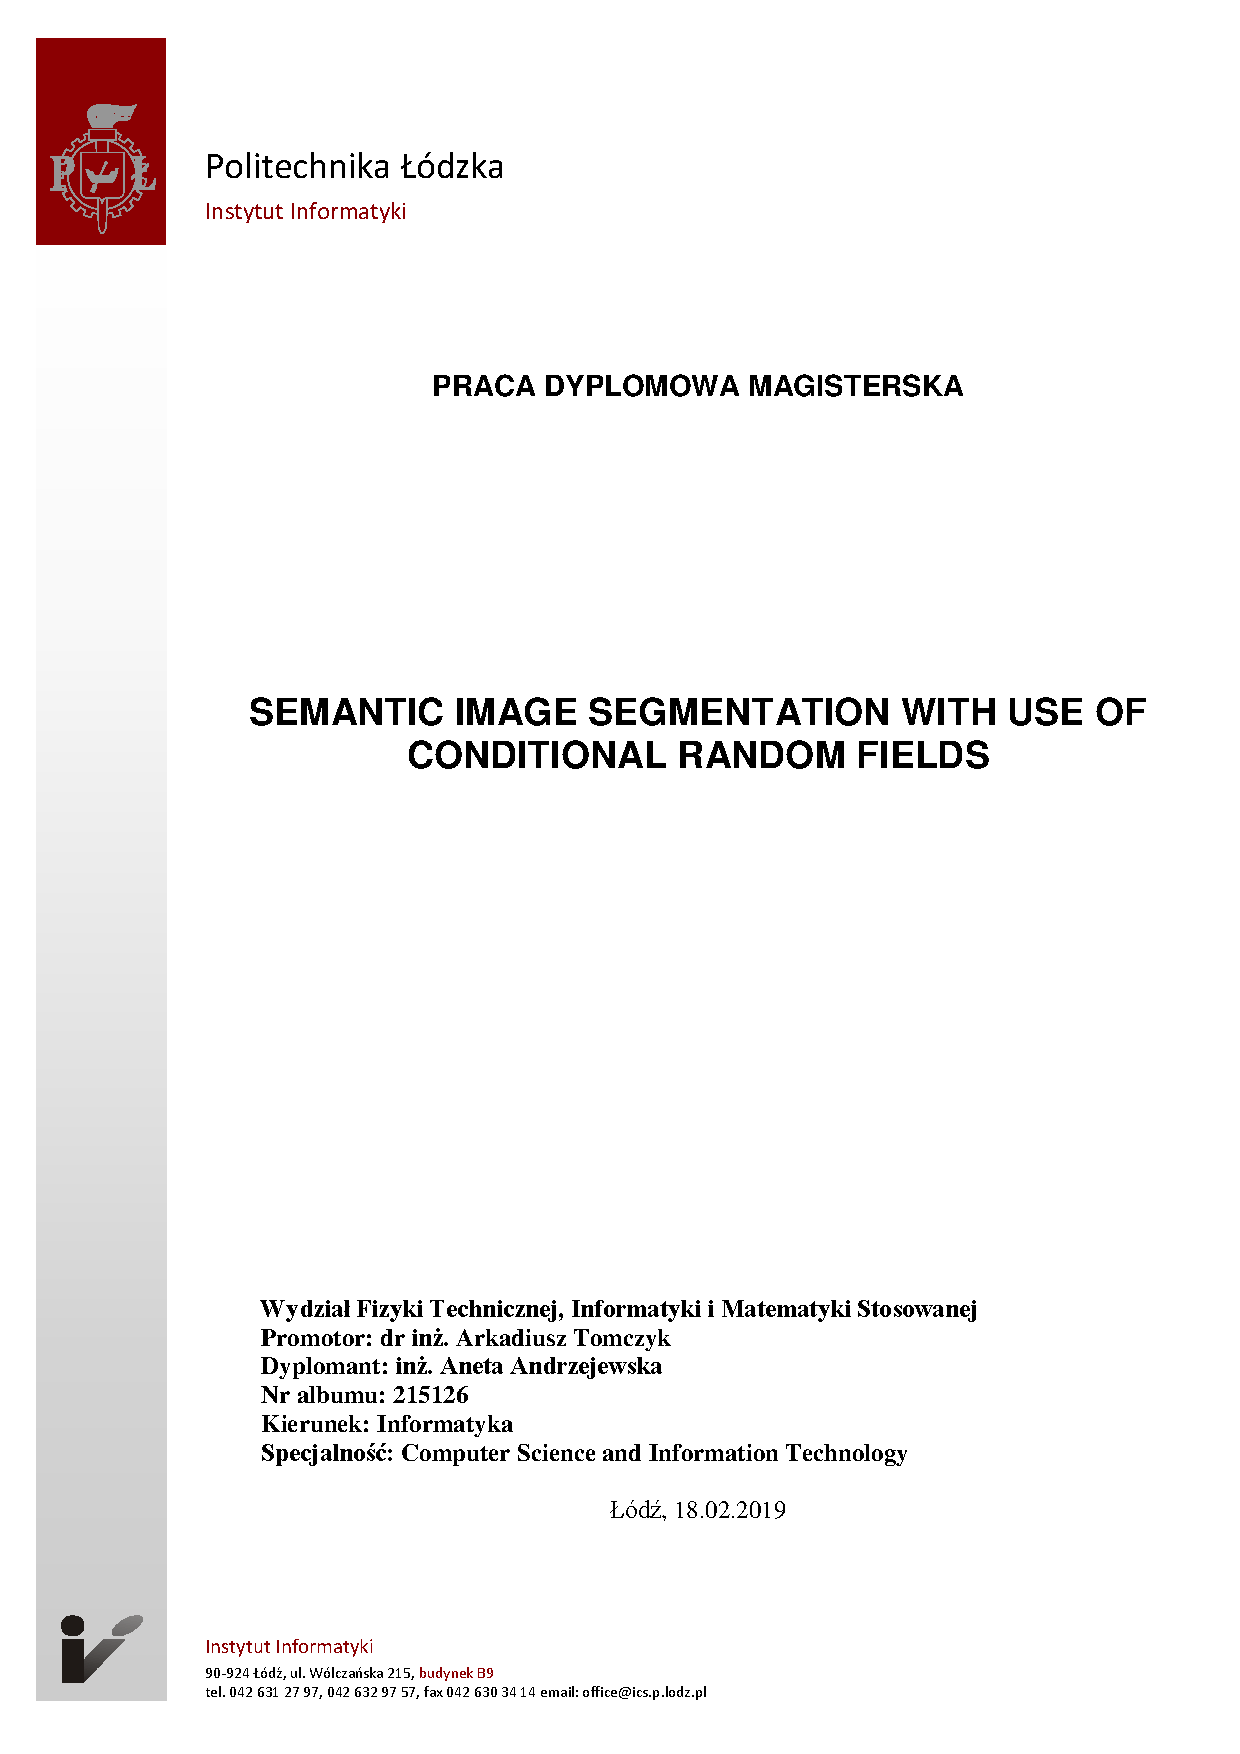
\includepdf[pages=-]{title_page_mgr.pdf}
\end{titlepage}



\import{sections/}{abstract}


\tableofcontents
\newpage

\chapter{Introduction}
\import{sections/introduction/}{introduction}

\section{Purpose and scope of the thesis}
\import{sections/introduction/}{purpose}

\section{Goals of the thesis}
\import{sections/introduction/}{goal}

\section{Thesis contents}
\import{sections/introduction/}{contents}

\chapter{Image Segmentation}
\import{sections/image_segmentation/}{introduction}

\section{Semantic Image Segmentation}
\import{sections/image_segmentation/}{semantic_segmentation}

\section{Semantic Image Segmentation methods}
\import{sections/image_segmentation/}{semantic_segmentation_methods}

\chapter{Structured Prediction}
\label{chapter:structured_prediction}
\import{sections/structured_prediction/}{introduction}

\section{Probabilistic Graphical Model}
\import{sections/structured_prediction/}{pgm}

\section{Factorisation}
\import{sections/structured_prediction/}{factorisation}

\section{Conditional Random Fields }
\import{sections/structured_prediction/}{crf}
	
\section{Inference in factor graphs}
\label{sec:inference}
\import{sections/structured_prediction/}{inference}

\section{Parameter training }
\import{sections/structured_prediction/}{parameter_training}

\section{Energy formulation}	
\label{sec:energy}
\import{sections/structured_prediction/}{energy}

\chapter{Semantic Image Segmentation system}
\import{sections/implementation_details/}{introduction}

\section{Dataset}	
\import{sections/implementation_details/}{dataset}

\section{Preprocessing}	
\import{sections/implementation_details/}{preprocessing}


\newpage
\printbibliography 
\end{document}
